% !TeX program = xelatex
\documentclass[10pt]{beamer}

\usetheme{metropolis}

\usepackage{pgfplots}
\usepgfplotslibrary{fillbetween}
\usepackage{pgfopts}
\usepackage{amsmath}
%\usepackage{structuralanalysis}
\usepackage{tikz}
\usepackage{tikz-3dplot}
\usepackage{chngcntr}
\usepackage{wasysym}
\usepackage{mathtools}
\usepackage{alphalph}
\usepackage{xcolor}
\usepackage[showdow=false, en-US]{datetime2}
\usepackage{hyperref}

\newcommand{\highlight}[1]{%
	\colorbox{red!50}{$\displaystyle#1$}}

\setcounter{lecture}{24}
\counterwithin{equation}{lecture}
\makeatletter
\def\user@resume{resume}
\def\user@intermezzo{intermezzo}
%
\newcounter{previousequation}
\newcounter{lastsubequation}
\newcounter{savedparentequation}
\setcounter{savedparentequation}{1}
% 
\renewenvironment{subequations}[1][]{%
	\def\user@decides{#1}%
	\setcounter{previousequation}{\value{equation}}%
	\ifx\user@decides\user@resume 
	\setcounter{equation}{\value{savedparentequation}}%
	\else  
	\ifx\user@decides\user@intermezzo
	\refstepcounter{equation}%
	\else
	\setcounter{lastsubequation}{0}%
	\refstepcounter{equation}%
	\fi\fi
	\protected@edef\theHparentequation{%
		\@ifundefined {theHequation}\theequation \theHequation}%
	\protected@edef\theparentequation{\theequation}%
	\setcounter{parentequation}{\value{equation}}%
	\ifx\user@decides\user@resume 
	\setcounter{equation}{\value{lastsubequation}}%
	\else
	\setcounter{equation}{0}%
	\fi
	\def\theequation  {\theparentequation  \alph{equation}}%
	\def\theHequation {\theHparentequation \alph{equation}}%
	\ignorespaces
}{%
%  \arabic{equation};\arabic{savedparentequation};\arabic{lastsubequation}
\ifx\user@decides\user@resume
\setcounter{lastsubequation}{\value{equation}}%
\setcounter{equation}{\value{previousequation}}%
\else
\ifx\user@decides\user@intermezzo
\setcounter{equation}{\value{parentequation}}%
\else
\setcounter{lastsubequation}{\value{equation}}%
\setcounter{savedparentequation}{\value{parentequation}}%
\setcounter{equation}{\value{parentequation}}%
\fi\fi
%  \arabic{equation};\arabic{savedparentequation};\arabic{lastsubequation}
\ignorespacesafterend
}
\makeatother
\title{AE 737 - Mechanics of Damage Tolerance}
\subtitle{Lecture \arabic{lecture}}
\date{Last Updated: \today\ at \DTMcurrenttime}
\author{Dr. Nicholas Smith}
\institute{Wichita State University, Department of Aerospace Engineering}
% \titlegraphic{\hfill\includegraphics[height=1.5cm]{logo/logo}}

\begin{document}
	
	\maketitle
	\begin{frame}{schedule}
		\begin{itemize}
			\item 26 Apr - Exam Solutions, Damage Tolerance
			\item 28 Apr - SPTE, Finite Elements
			\item 3 May - Damage in Composites
			\item 5 May - Repair, Final Project Due May 10
		\end{itemize}
	\end{frame}
	
	\begin{frame}
		\frametitle{outline}
		\setbeamertemplate{section in toc}[sections numbered]
		\tableofcontents[hideallsubsections]
	\end{frame}

	\section{exam}
	\begin{frame}{exam}
		\begin{itemize}
			\item Class average: 89.5
			\item Standard deviation: 11%
			\item There is no curve for this exam
		\end{itemize}
	\end{frame}
	
	\begin{frame}<handout:0>{solutions}
		
	\end{frame}
	
	\section{damage tolerance}
	
	\begin{frame}{definitions}
		\begin{itemize}[<+->]
			\item \textbf{Safe Life}
			\begin{itemize}
				\item Assume cracks are present
				\item Cracks are not inspectable
				\item Use crack growth or fatigue analysis to establish safe life, in which part will not fail
			\end{itemize}
			\item \textbf{Damage tolerant}
			\begin{itemize}
				\item Assume cracks are present
				\item When cracks grow to a sufficient size, they are inpsectable
				\item Inspection cycles are set such that we can be sure crack will not become critical during regular operation
			\end{itemize}
		\end{itemize}
	\end{frame}
	
	\begin{frame}{definitions}
		\begin{itemize}[<+->]
			\item \textbf{Fail safe} multiple load paths, redundancy 
			\item \textbf{Limit load} maximum anticipated load
			\item \textbf{Design load} limit load multiplied by some factor of safety (static design)
			\item \textbf{Operating load} stress spectrum (used for crack propagation/fatigue)
		\end{itemize}
	\end{frame}
	
	\begin{frame}{structural categories}
		\begin{itemize}[<+->]
			\item Single load path - safe life
			\item Single load path - damage tolerant
			\item Multiple load path - externally inspectable
			\item Multiple load path - inspectable prior to failure
		\end{itemize}
	\end{frame}
	
	\begin{frame}{single load path - safe life}
		\begin{itemize}[<+->]
			\item In many structures, multiple load paths are not practical
			\item It is also possible for the critical crack length to be much smaller than is easily detectable
			\item In these cases, safe life design is used to identify a certain number of cycles a part can sustain before it needs to be replaced
			\item This often requires replacing parts pre-maturely
		\end{itemize}
	\end{frame}
	
	\begin{frame}{single load path - damage tolerant}
		\begin{itemize}[<+->]
			\item Redundant load paths are not necessary when a part is easily inspectable
			\item When the detectable crack size is much less than the critical crack length, we can safely inspect a part so that it is only replaced when damage is detected
			\item Many times this damage can be repaired to avoid replacing the part entirely
			\item Ideal for large, expensive parts that are easy to access (inspection and repair)
		\end{itemize}
	\end{frame}
	
	\begin{frame}{multiple load path - externally inspectable}
		\begin{itemize}[<+->]
			\item This is a very common scenario in aircraft (skin/stringer)
			\item In this case, the primary structure is not inspectable
			\item A secondary structure is inspectable
			\item The secondary structure can support a certain number of cycles after failure of the primary structure
			\item Secondary structure can be inspected to observe damage in primary structure
		\end{itemize}
	\end{frame}
	
	\begin{frame}{multiple load path - inspectable prior to failure}
		\begin{itemize}[<+->]
			\item In this case the primary structure is inspectable
			\item Otherwise same as externally inspectable structure
		\end{itemize}
	\end{frame}
	
	\section{inpsection cycle}
	
	\begin{frame}{inspection cycle}
		\begin{itemize}[<+->]
			\item In many industries, an inspection cycle is pre-determined by some governing agency
			\item We have developed all the equations necessary to determine our own
			\begin{enumerate}
				\item Determine loading cycle (or equivalent load cycle using Boeing method)
				\item Determine maximum crack length
				\item Determine initial assumed crack length (minimum detectable crack)
				\item Calculate number of cycles/flights until crack grows to maximum allowable size
			\end{enumerate}
		\end{itemize}
	\end{frame}
	
	\begin{frame}{load cycle}
		\begin{itemize}[<+->]
			\item Be sure to use a consistent cycle-counting method (rainflow or range-pair)
			\item Recall the Boeing method for variable amplitude loads
			\item[] \begin{equation}
			\sum_i \left( z\sigma_{max} \right)_i^{p}N_i = \left( S \right)^{p}
			\end{equation}	
		\end{itemize}
	\end{frame}
	
	\begin{frame}{crack length}
		\begin{itemize}[<+->]
			\item We can use the residual strength curve to set a maximum crack length
			\item We also want to ensure that the crack propagation is still in Region II at this point
			\item Crack growth becomes unstable in Region III
		\end{itemize}
	\end{frame}
	
	\begin{frame}{initial crack length}
		\begin{itemize}[<+->]
			\item What is the smallest crack we can detect?
			\item Liquid penetrant (any material)
			\item Magnetic particle (ferromagnetic materials)
			\item Ultrasonic (any material)
			\item Eddy Current (only for conductive materials)
			\item Radiographic (X-Ray, nearly any material)
		\end{itemize}
	\end{frame}
	
	\begin{frame}{calculate cycles}
		\begin{itemize}[<+->]
			\item We can integrate (analytically or numerically) to find the number of cycles it will take for a crack to grow to critical length
			\item Note that numerical integration is non-conservative, in general
			\item $\Delta N$ should be small enough to give converged solution
		\end{itemize}
	\end{frame}
	
	\begin{frame}{example}
		
	\end{frame}
	
	\section{finite elements}
	
	\begin{frame}{finite element methods in fracture}
		\begin{itemize}[<+->]
			\item Direct method (use near-tip stress field)
			\begin{itemize}
				\item Requires very fine mesh near the tip to be accurate
				\item Can be made feasible with specialty elements
			\end{itemize}
			\item Crack closure method
			\begin{itemize}
				\item An energy based method
				\item Calculate energy to close crack one element away from crack tip
				\item Can have a courser mesh than direct method
			\end{itemize}
			\item Cohesive elements
			\begin{itemize}
				\item Specialty elements act like an adhesive between two materials
				\item Used to model crack propagation when crack path (and material behavior) are known
			\end{itemize}
			\item XFEM
			\begin{itemize}
				\item eXtended Finite Element Method
				\item Can predict crack growth in any direction
				\item Adds "phantom" cracks in all elements
			\end{itemize}
		\end{itemize}
	\end{frame}
	
	%TODO: direct method (specialty elements)
	\begin{frame}{direct method}
		\begin{itemize}[<+->]
			\item We already know that the stress field near the crack tip is
			\begin{equation*}
			\sigma_{yy} = \frac{K_I}{\sqrt{2 \pi x}}
			\end{equation*}
			\item We can solve this for $K_I$ and we should (in theory) be able to calculate $K_I$
			\item We will get a unique $K_I$ value for every point ($x$) along crack plane
			\item For this method to be accurate, we need to capture the singularity at crack tip
			\item This requires a very fine mesh (computationally expensive)
			\item Alternatively, many FE packages include "singularity" elements which allow coarse(r) mesh
		\end{itemize}
	\end{frame}
	
	\begin{frame}{modeling tips}
		\begin{itemize}[<+->]
			\item Use symmetry in your model to reduce node count
			\item Center-crack can be modeled using on 1/4 of the model
			\item Use biased node seeding (more nodes near tip)
		\end{itemize}
	\end{frame}
	
	\begin{frame}{symmetry}
		\begin{figure}
			\centering
			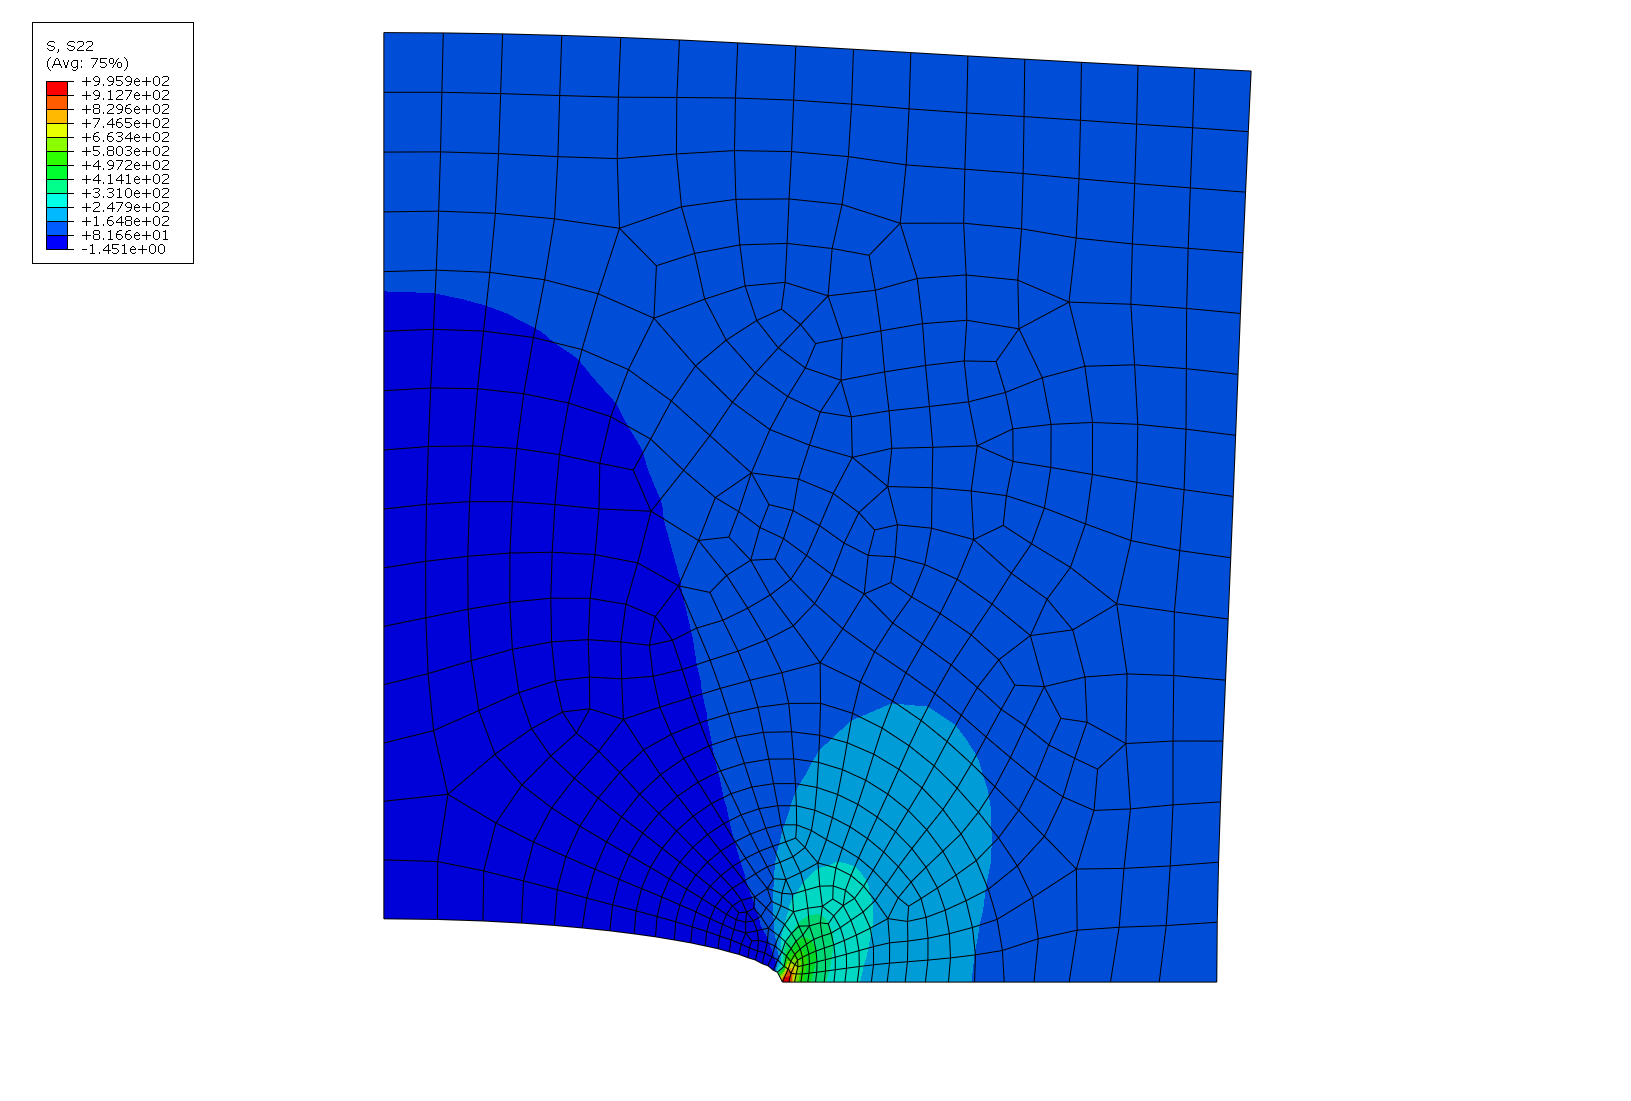
\includegraphics[width=0.7\linewidth]{../Figures/singularity_quarter}
			\caption{}
			\label{fig:singularity_quarter}
		\end{figure}
	\end{frame}
	
	\begin{frame}{symmetry}
		\begin{figure}
		\centering
		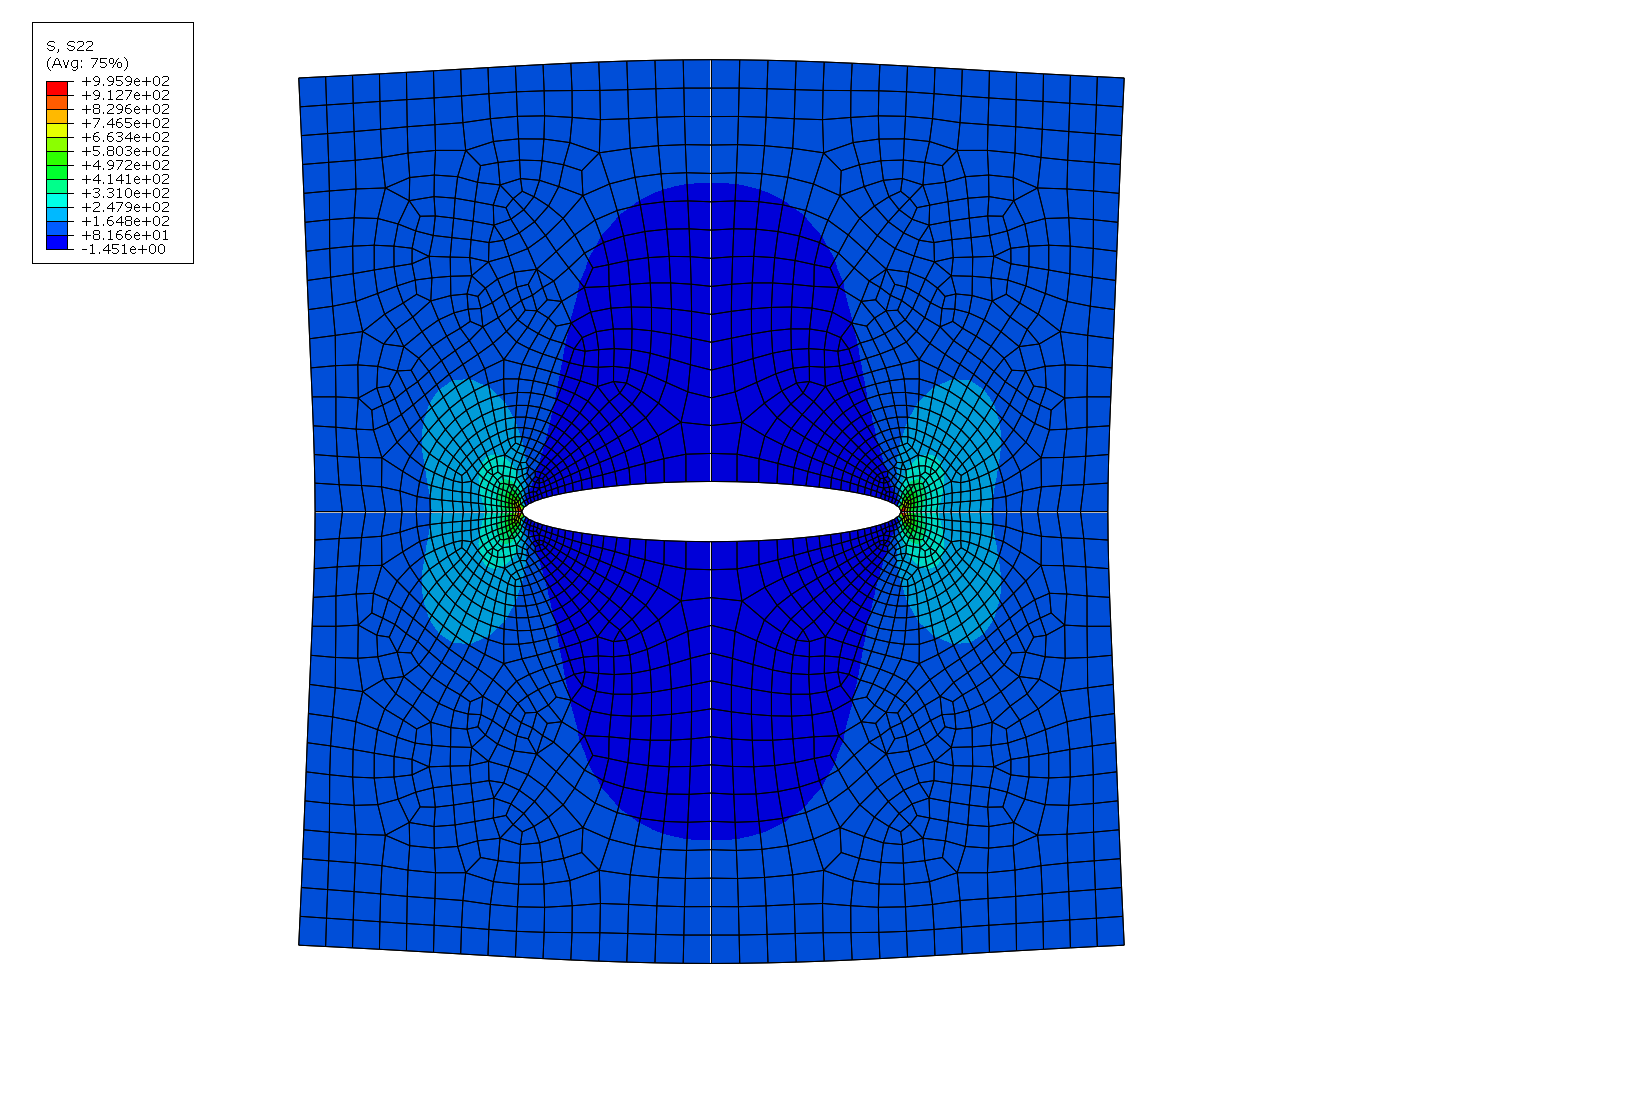
\includegraphics[width=0.7\linewidth]{../Figures/singularity_mirrored}
		\caption{}
		\label{fig:singularity_mirrored}
		\end{figure}
	\end{frame}
	
	\begin{frame}{analyzing results}
		\begin{itemize}[<+->]
			\item If our results are accurate, we should be able to calculate the same $K_I$ at any point
			\item To ensure convergence, we plot the calculated $K_I$ vs. $x$ (distance from crack tip)
			\item In the region where this plot is a horizontal line, we consider a converged $K_I$
			\item It is also possible to consider the crack opening displacement
			\begin{equation*}
			u_y = \frac{K_I(\kappa + 1)}{4 \nu \pi}\sqrt{-2 \pi x}
			\end{equation*}
			\item Where $\kappa$ is to easily differentiate between plane stress and plane strain
			\begin{align*}
			\kappa &= 3 - 4\nu & \text{(plane strain)}\\
			\kappa &= \frac{3-\nu}{1+\nu} & \text{(plane stress)}
			\end{align*}
			\item The displacement method is generally more accurate in Finite Elements
		\end{itemize}
	\end{frame}
	
	\begin{frame}{stress results}
		\begin{tikzpicture}
		\begin{axis}[
		xmin=0, xmax=1.2,
		ymin=200, ymax=1000,
		axis y line*=left,
		yticklabel style=blue,
		ylabel style=blue,
		y axis line style=blue,
		ytick style=blue,
		xlabel=x,
		ylabel={$\sigma$},
		ylabel near ticks]
		\addplot [color=blue]
			table[x=x,y=s22] {s22.txt};
		\end{axis}
		\begin{axis}[
		xmin=0, xmax=1.2,
		ymin=400, ymax=800,
		axis y line*=right,
		yticklabel style=red,
		ylabel style=red,
		y axis line style=red,
		ytick style=red,
		xlabel=x,
		ylabel={$K_I$},
		ylabel near ticks]
		\addplot [color=red]
			table[x=x,y=KI] {s22.txt};
		\end{axis}
		\end{tikzpicture}
	\end{frame}
	
	\begin{frame}{displacement results}
		\begin{tikzpicture}
		\begin{axis}[
		xmin=0, xmax=1.2,
		ymin=0, ymax=0.1,
		axis y line*=left,
		yticklabel style=blue,
		ylabel style=blue,
		y axis line style=blue,
		ytick style=blue,
		xlabel=x,
		ylabel={$u_y$},
		ylabel near ticks]
		\addplot [color=blue]
		table[x=x,y=u2] {u2.txt};
		\end{axis}
		\begin{axis}[
		xmin=0, xmax=1.2,
		ymin=400, ymax=800,
		axis y line*=right,
		yticklabel style=red,
		ylabel style=red,
		y axis line style=red,
		ytick style=red,
		xlabel=x,
		ylabel={$K_I$},
		ylabel near ticks]
		\addplot [color=red]
		table[x=x,y=KI] {u2.txt};
		\end{axis}
		\end{tikzpicture}
	\end{frame}
	
	\begin{frame}{next class}
		\begin{itemize}
			\item crack closure
			\item cohesive elements
			\item XFEM
			\item damage in composites
		\end{itemize}
	\end{frame}
	%TODO: crack closure methods (chapter 4 in fracture text)
	%TODO: cohesive elements (chapter 9 in fracture text)
	%TODO: XFEM
\end{document}
